\documentclass[12pt,a4paper]{report}
\usepackage{graphicx}
\usepackage{hyperref}
\usepackage{amsmath}
\usepackage{float}
\usepackage{geometry}
\geometry{margin=1in}

\begin{document}


\begin{titlepage}
\centering
\vspace*{2cm}
\Huge\textbf{Technical Report: GetClasses System}\\[0.5cm]
\Large\textit{An Object-Oriented Transactional Application for Online Tutoring (Work in Progress)}\\[2cm]
\Large\textbf{Authors:}\\[0.2cm]
Jhon Gonzalez, Alejandro Escobar, Sebasti\'an Zambrano\\[0.3cm]
Computer Engineering Program\\
Universidad Distrital Francisco Jos\'e de Caldas\\[0.3cm]
\\[2cm]
\Large\textbf{Instructor:} Eng. Carlos Andr\'es Sierra, M.Sc.\\[1cm]
\Large\textbf{Date:} October 2025\\[2cm]
\vfill
\end{titlepage}



\begin{abstract}
This technical report presents the initial version of GetClasses, an object-oriented transactional system designed to connect students and tutors through a secure, modular, and scalable software architecture. The system is being developed in Java using JavaFX as the graphical interface framework and follows a layered architecture with SOLID principles. At this stage, the project includes preliminary implementations of user registration, scheduling management, and file-based persistence. Future work will extend the system with communication, payment simulation, and review functionalities. The document details the current progress, design structure, and the roadmap for completing pending modules.
\end{abstract}

\tableofcontents
\listoffigures
\listoftables
\newpage

\chapter{Introduction}
The growing demand for flexible and remote education has motivated the development of systems that facilitate personalized tutoring experiences. GetClasses aims to provide a digital environment where students can connect with tutors, schedule sessions, and exchange information efficiently.


Currently, many existing platforms—such as Coursera or Udemy—focus on course distribution rather than real-time tutoring interactions. The objective of GetClasses is to fill this gap through a transactional system that integrates user management, scheduling, and communication tools.


This report summarizes the current state of the project, the applied methodologies, and the components that are still under development.


\chapter{Literature Review}
Research on online education platforms highlights challenges such as scalability, security, and personalized user experiences. While established platforms manage large amounts of data efficiently, they often lack direct tutor-student interaction. Studies in software engineering emphasize that object-oriented programming (OOP), layered architecture, and SOLID principles are effective strategies for building modular and maintainable educational software systems \cite{b1,b2,b3}.


The GetClasses project is based on these methodologies, combining theoretical foundations with a practical software prototype.


\chapter{Background}
This project originated from the Object-Oriented Programming course at Universidad Distrital Francisco Jos\'e de Caldas. It consolidates concepts from several academic workshops focused on conceptual design, UML modeling, inheritance and polymorphism, and SOLID-based architecture refinement.


The project uses JavaFX to develop the user interface and file-based persistence for data storage. Future iterations are expected to include a database-driven persistence layer, enhanced authentication, and integrated messaging features.


\chapter{Objectives}
\section{General Objective}
To design and progressively implement a transactional application connecting tutors and students using object-oriented programming principles and layered software architecture.

\section{Specific Objectives}
\begin{itemize}
    \item Apply OOP principles such as encapsulation, inheritance, and polymorphism.
    \item Design a clear and scalable class hierarchy following SOLID principles.
    \item Implement a JavaFX-based interface for registration and session scheduling.
    \item Develop file-based data persistence as an initial storage mechanism.
    \item Evaluate system functionality through incremental testing phases.
\end{itemize}


\chapter{Scope}
At this stage, GetClasses focuses on the implementation of core structural components, including:
\begin{itemize}
    \item User class hierarchy (Student, Tutor, Admin).
    \item Basic registration and login process.
    \item Preliminary scheduling logic and persistence prototype.
\end{itemize}


Functionalities such as chat, payment simulation, and user reviews are planned for future versions. The current version serves as a foundation for expansion and future deployment as a full tutoring platform.

\chapter{Assumptions and Limitations}
\section{Assumptions}
\begin{itemize}
    \item Users are familiar with basic digital platforms.
    \item Tutors provide accurate subject and availability data.
    \item Local file storage is consistent between sessions.
\end{itemize}


\section{Limitations}
\begin{itemize}
    \item Some modules are still in early stages of development.
    \item Communication and payment systems are not yet integrated.
    \item Testing results are preliminary and limited to isolated functions.
    \item File-based persistence restricts scalability and data integrity.
\end{itemize}


\chapter{Methodology}
The project follows an iterative and incremental software development process, with continuous feedback and improvement. Each cycle includes design refinement, coding, and functional testing of individual components.

\section{System Architecture}
The GetClasses architecture is organized into three layers:
\begin{itemize}
    \item \textbf{Presentation Layer:} Built with JavaFX, it manages user interaction and visualization.
    \item \textbf{Business Logic Layer:} Contains service classes for registration, scheduling, and system control.
    \item \textbf{Data Layer:} Manages file serialization and data retrieval operations.
\end{itemize}


\newpage


\section{Class Design}
The conceptual model defines a superclass \texttt{User}, extended by subclasses \texttt{StudentUser}, \texttt{TutorUser}, and \texttt{AdminUser}. Each subclass introduces role-specific behavior, maintaining encapsulation and reusability.

\begin{figure}[H]
    \centering
    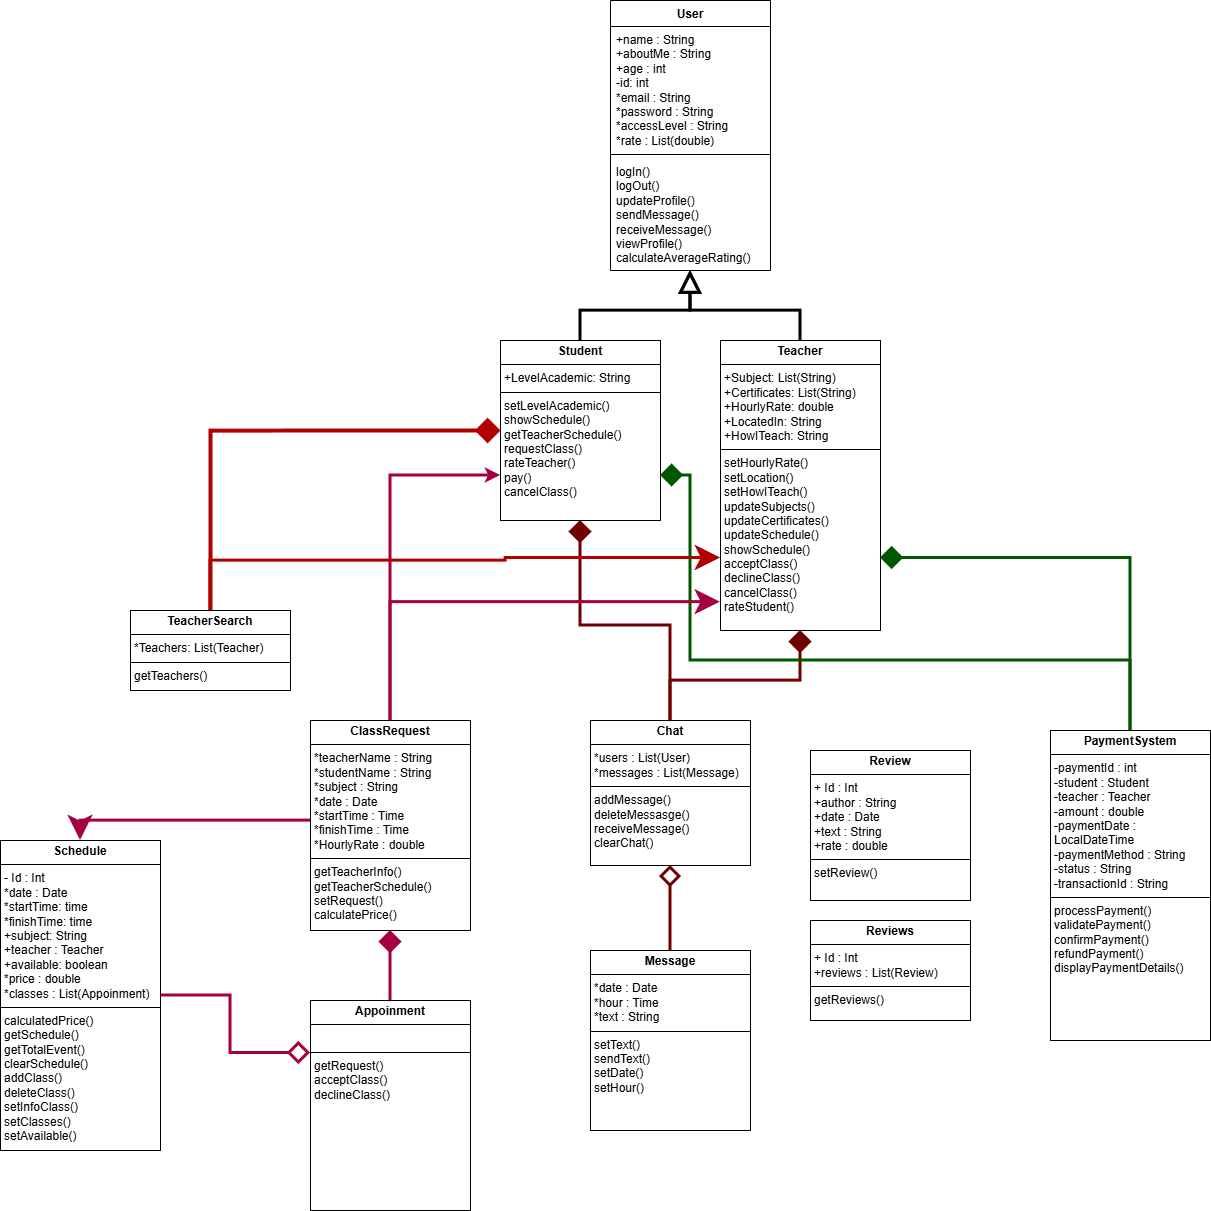
\includegraphics[width=1.0\textwidth]{UML.png}
    \caption{UML class diagram showing inheritance and associations.}
    \label{fig:uml}
\end{figure}


\chapter{Preliminary Results}
At this stage, only partial testing has been conducted on user registration and file-based persistence. The following table summarizes the preliminary outcomes:


\begin{table}[H]
\centering
\caption{Preliminary testing summary}
\begin{tabular}{|l|c|l|}
\hline
\textbf{Test Module} & \textbf{Status} & \textbf{Description} \\
\hline
User Registration & In Progress & Users can register and store data in files. \\
\hline
Login Function & In Progress & Partial functionality; missing validation layer. \\
\hline
Review System & In Progress & Initial structure created; functionality under development. \\
\hline
Scheduling System & In Progress & To be implemented in the next iteration. \\
\hline
Chat Module & Pending & Not yet developed. \\
\hline
Payment Simulation & Pending & Planned for final stage. \\
\hline

\end{tabular}
\label{tab:results}
\end{table}



Initial results indicate that the system correctly stores and retrieves user data using file serialization. No major errors have been detected in these early modules.

\chapter{Discussion}
The development of GetClasses demonstrates how object-oriented principles can be applied progressively in a real-world educational context. Even though several modules remain under construction, the current design ensures modularity, maintainability, and future scalability.


Challenges include managing dependencies between layers and implementing a more efficient persistence model. Once database integration and user communication are completed, the system will achieve a more realistic and functional structure.

\chapter{Future Work and Conclusions}
\section{Future Work}
\begin{itemize}
    \item Implement full scheduling, chat, and payment modules.
    \item Replace file-based persistence with a relational or NoSQL database.
    \item Add user interface improvements using advanced JavaFX components.
    \item Conduct complete unit and integration testing.
    \item Explore web or mobile deployment options.
\end{itemize}


\section{Conclusions}
Although GetClasses is still under active development, the project demonstrates solid progress in design and foundational architecture. It successfully applies OOP and SOLID principles to create a maintainable software structure. Future implementations will expand its features and provide a comprehensive platform for online tutoring.


\begin{thebibliography}{99}
\bibitem{b1} I. Sommerville, \textit{Software Engineering}, 10th ed., Pearson, 2015.
\bibitem{b2} K. Beck and M. Fowler, \textit{Planning Extreme Programming}, Addison-Wesley, 2000.
\bibitem{b3} S. W. Ambler, \textit{Agile Modeling: UML Diagrams and Class Design}, AgileModeling.com, 2023.
\bibitem{b4} P. Coad and E. Yourdon, \textit{Object-Oriented Design}, Prentice Hall, 1991.
\bibitem{b5} IEEE Standards Association, \textit{Guide to Software Design Documentation (IEEE 1016-2020)}, 2023.
\end{thebibliography}


\appendix



\chapter{Mockups and Interfaces}
\section{Mockups}
\begin{figure}[h!]
\centering
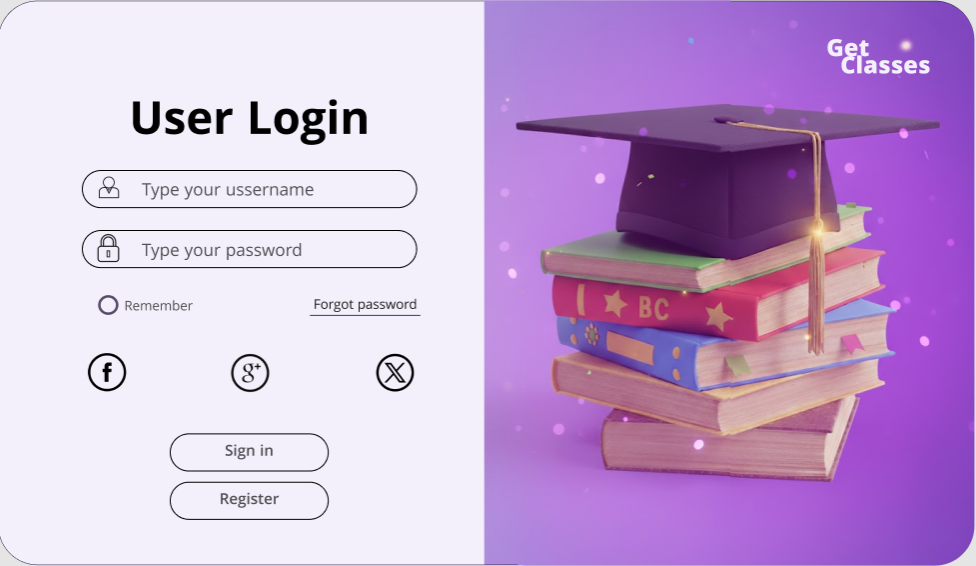
\includegraphics[width=0.8\textwidth]{LoginScreen.png}
\caption{Login Page}
\end{figure}


\begin{figure}[h!]
\centering
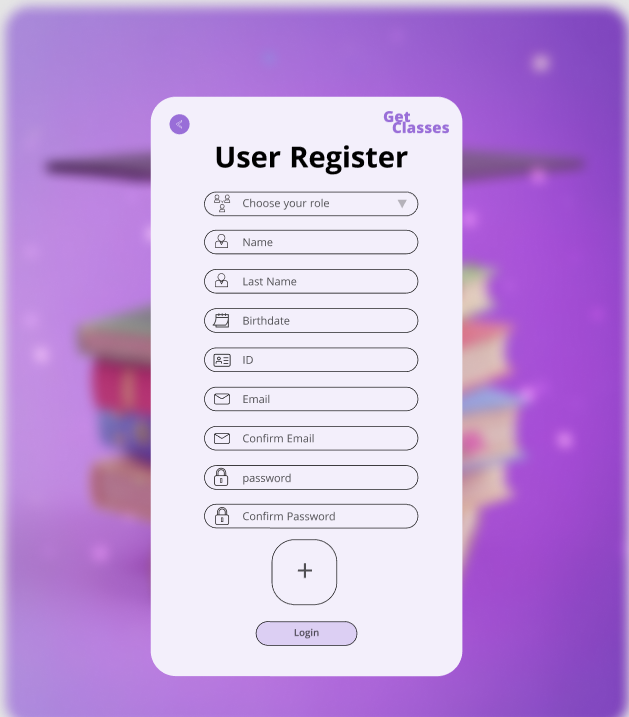
\includegraphics[width=0.6\textwidth]{RegisterScreen.png}
\caption{Register Page}
\end{figure}

        
\newpage


\begin{figure}[h!]
\centering
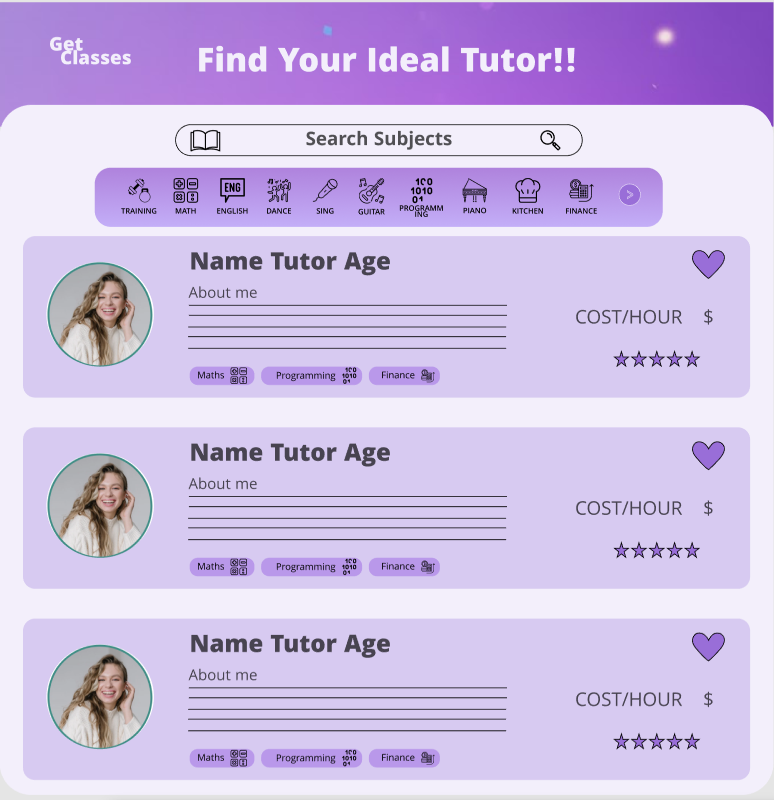
\includegraphics[width=0.7\textwidth]{MainScreen.png}
\caption{Main Page}
\end{figure}


\begin{figure}[h!]
\centering
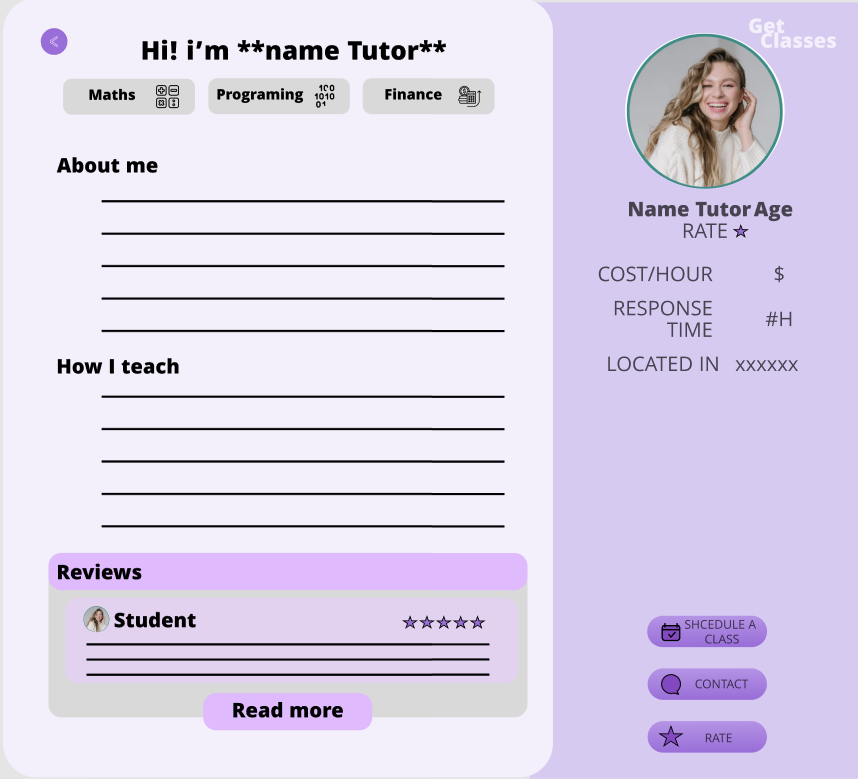
\includegraphics[width=0.6\textwidth]{ProfileTutorScreen.png}
\caption{tutor profile Page}
\end{figure}

\newpage


\begin{figure}[h!]
\centering
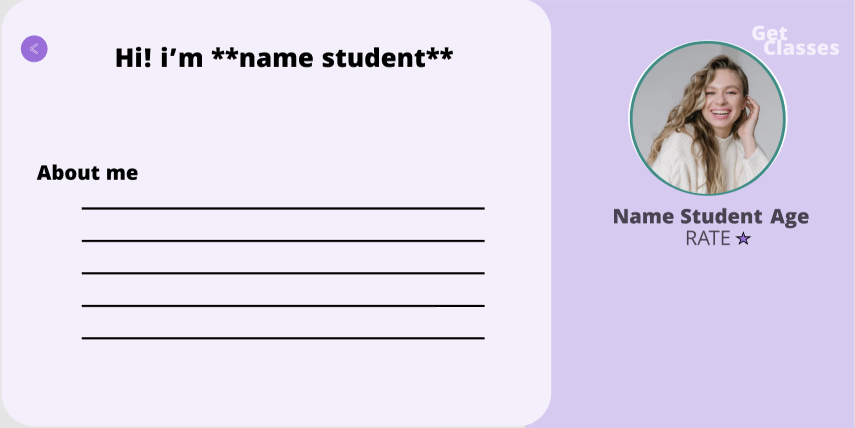
\includegraphics[width=0.8\textwidth]{ProfileStudentScreen.png}
\caption{Student Profile Page}
\end{figure}


\begin{figure}[h!]
\centering
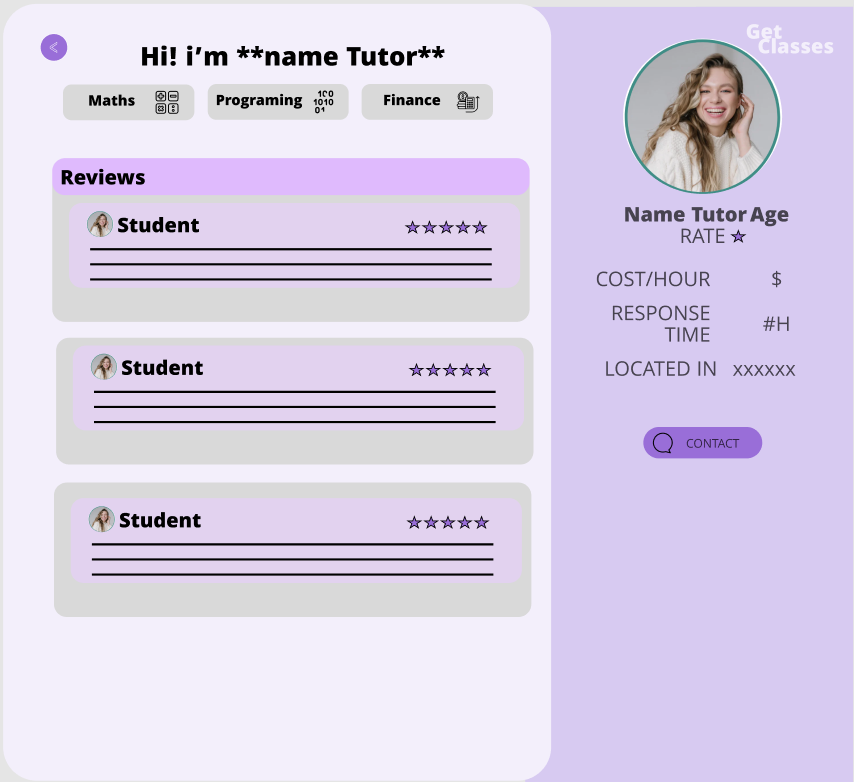
\includegraphics[width=0.8\textwidth]{ReviewsScreen.png}
\caption{Review List Page}
\end{figure}


\newpage


\begin{figure}[h!]
\centering
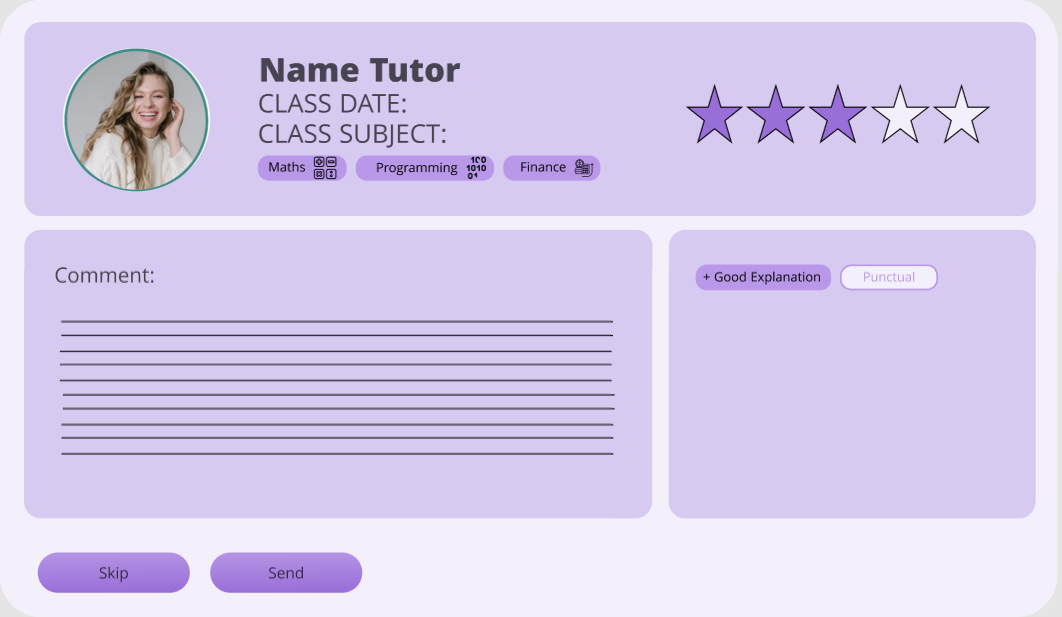
\includegraphics[width=0.8\textwidth]{ReviewScreen.png}
\caption{Make Review page}
\end{figure}



\begin{figure}[h!]
\centering
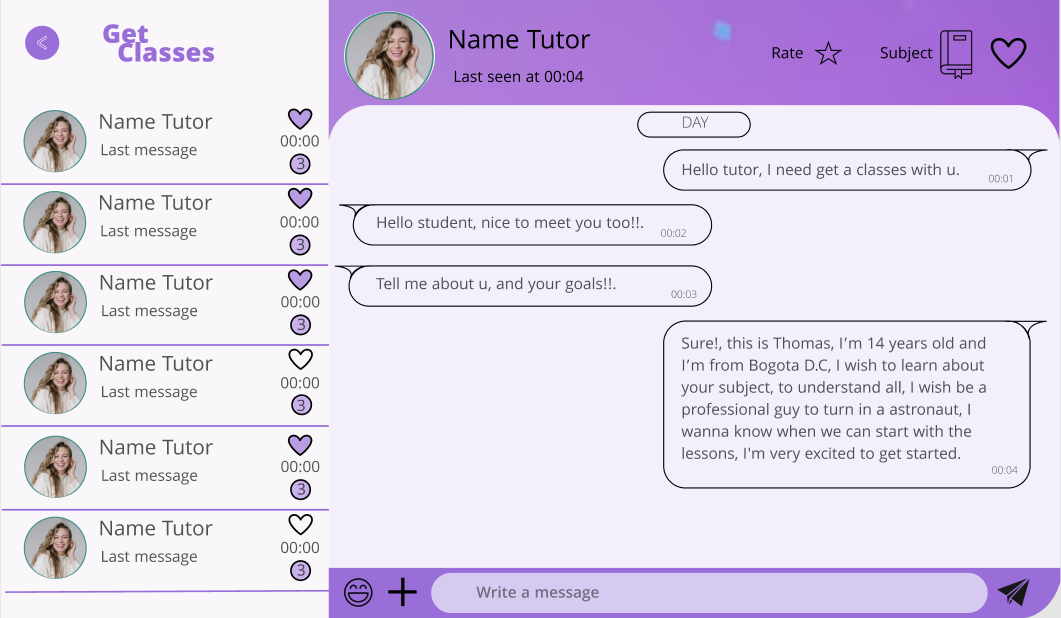
\includegraphics[width=0.8 \textwidth]{ChatScreen.png}
\caption{Chat Page}
\end{figure}


\newpage


\chapter{Glossary}
\begin{description}
    \item[OOP] Object-Oriented Programming.
    \item[SOLID] A set of design principles for clean, maintainable code.
    \item[UML] Unified Modeling Language for software system design.
    \item[JavaFX] A graphical framework for building Java-based GUI applications.
\end{description}


\end{document}